\documentclass[tikz,border=0pt]{standalone}
\usepackage[T1]{fontenc}
\usepackage{helvet}
\renewcommand{\familydefault}{\sfdefault}
% Reuse accepted label-free artwork through vector viewports; no pixel editing.
\usepackage{graphicx}
\usetikzlibrary{arrows.meta,calc}
\tikzset{flow/.style={-{Stealth[length=1.6mm,width=1.1mm]},line width=.75pt},
 wirelabel/.style={fill=white,inner sep=1.2mm},
 every node/.style={font=\fontsize{9}{11}\selectfont,align=center,inner sep=1pt}}
% Arguments: source left/top/right/bottom pixels; destination left/bottom/width mm.
\newcommand{\artpiece}[7]{
 \pgfmathsetmacro{\pieceScale}{#7/((#3-#1)*.1)}
 \begin{scope}[shift={(#5,#6)},scale=\pieceScale,transform shape]
  \clip (0,0) rectangle ({(#3-#1)*.1},{(#4-#2)*.1});
  \node[anchor=south west,inner sep=0pt] at ({-#1*.1},{-(931-#4)*.1})
   {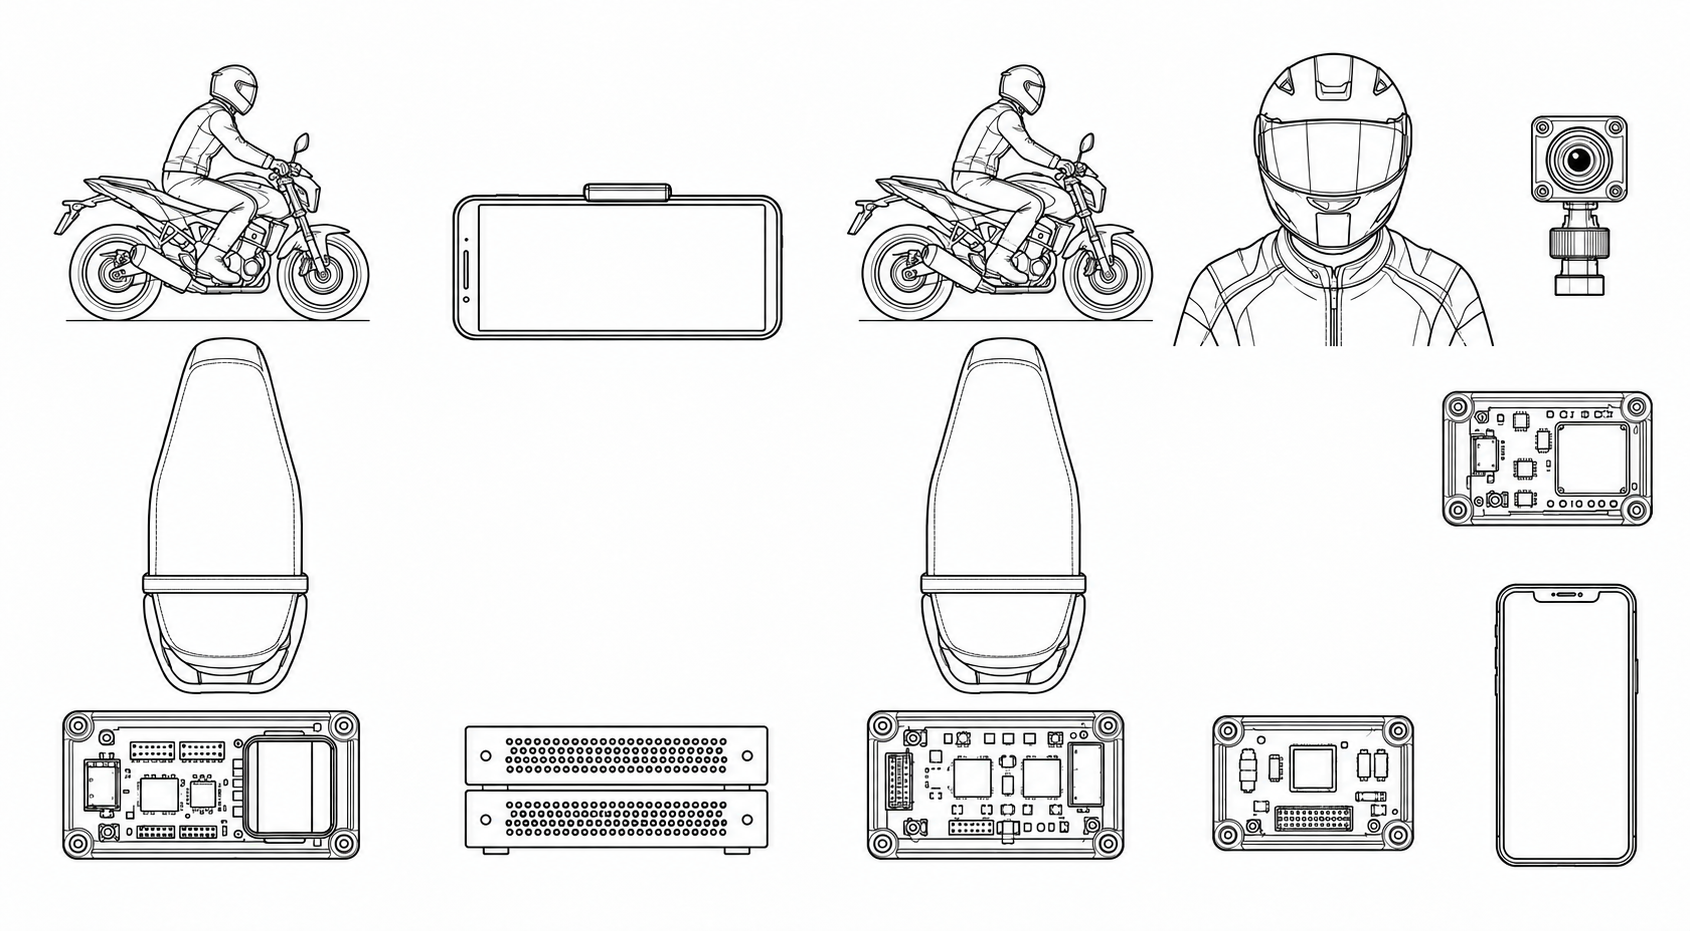
\includegraphics[width=169mm]{artwork-original.png}};
 \end{scope}}
\newcommand{\marker}[2]{
 \fill[white] (#1-2.4,#2-2.4) rectangle (#1+2.4,#2+2.4);
 \fill (#1-2,#2-2) rectangle (#1+2,#2+2);
 \fill[white] (#1-1.2,#2-1.2) rectangle (#1+1.2,#2+1.2);
 \fill (#1-1.2,#2-1.2) rectangle (#1,#2);
 \fill (#1,#2) rectangle (#1+1.2,#2+1.2);
}
\newcommand{\phoneglyph}[2]{
 \begin{scope}[shift={(#1,#2)}]
  \draw[densely dotted] (-8,0)--(8,0) (0,-13)--(0,13);
  \draw (0,10) .. controls (7,12) and (3,4) .. (7,-1)
    .. controls (11,-9) and (-4,-13) .. (-6,-7)
    .. controls (-9,0) and (-6,8) .. (0,10);
 \end{scope}}

\usetikzlibrary{patterns}
\begin{document}
\begin{tikzpicture}[x=1mm,y=1mm,line width=.65pt,line cap=round,line join=round]
\path[use as bounding box] (0,0) rectangle (240,180);

\draw (8,101) rectangle (232,174);
\node[anchor=west] at (12,169) {A. 2017 / Human--Computer Interaction: INTERACT / implemented demonstration};
\artpiece{35}{48}{380}{328}{13}{121}{37}
\artpiece{130}{330}{315}{700}{61}{121}{16}
\foreach \xx in {66.5,71.5}{\draw[fill=white] (\xx-1,135) rectangle (\xx+1,137);}
\artpiece{55}{708}{370}{865}{91}{130}{31}
\artpiece{445}{178}{790}{345}{145}{127}{42}
\draw (150,134)--(155,134)--(155,141)--(160,141)--(160,132)--(165,132)--(165,137)--(172,137);
\draw (179,137) circle (3);\draw (179,140)--(179,137)--(182,136);
\artpiece{455}{720}{775}{860}{202}{129}{25}
\draw[flow] (50,134)--(61,134) (77,138)--(91,138) (122,138)--(145,138) (187,138)--(202,138);
\node[align=center] at (31,115) {Everyday\\motorbike ride};
\node[align=center] at (69,115) {2 force-sensitive\\seat resistors};
\node[align=center] at (106,115) {Genuino\\microcontroller};
\node[wirelabel,align=center] at (133,152) {Bluetooth\\Low Energy};
\node[align=center] at (166,115) {Past 3 minutes\\and whole-ride variation};
\node[align=center] at (214,115) {Remote\\retrieval};
\node at (120,105.5) {0--1023 readings / four pressure bins / live feedback followed by reflection};
\draw (8,28) rectangle (232,97);
\node[anchor=west] at (12,92) {B. 2019 / Tangible, Embedded and Embodied Interaction / Bike Area Network};
\artpiece{1170}{45}{1500}{345}{12}{50}{30}
\foreach \xx/\yy in {27/73.3,27/60.4,17/55.5,37.7/55.5}{\begin{scope}[shift={(\xx,\yy)},scale=.7]\marker{0}{0}\end{scope}}
\artpiece{130}{330}{315}{700}{55}{47}{17}
\foreach \yy in {62,67.5,73}{\foreach \xx in {61.1,65.9}{\draw[fill=white] (\xx,\yy) circle (.9);}}
\draw (88,64) rectangle (133,82) (88,40) rectangle (133,58);
\node[align=center] at (110.5,73) {Camera +\\Raspberry Pi};
\node[align=center] at (110.5,49) {Pressure conversion +\\Raspberry Pi};
\draw[flow] (42,70)--(47,70)--(47,85)--(84,85)--(84,78)--(88,78) (72,58)--(88,49);
\draw (154,50) rectangle (190,72);\node[align=center] at (172,61) {Central\\Raspberry Pi};
\draw[flow] (133,73)--(143,73)--(143,65)--(154,65) (133,49)--(143,49)--(143,56)--(154,56);
\artpiece{1490}{580}{1645}{868}{207}{44}{18}
\begin{scope}[shift={(216,61)},scale=.5]\phoneglyph{0}{0}\end{scope}
\draw[dashed] (216,66) ellipse (3.5 and 5.5);
\draw[flow] (190,61)--(207,61);
\node[wirelabel] at (148,83) {WebSockets};
\node[align=center] at (29,39) {4 tracked markers:\\helmet top, chin,\\both shoulders};
\node[align=center] at (63.5,33) {6 seat pressure sensors};
\node[align=center] at (172,39) {Combine load distribution\\with upper-body geometry};
\node at (216,39) {Glanceable contour};
\node at (148,31.5) {Modules reported; full integration, learning and ride evaluation proposed};
\draw (8,3) rectangle (232,24);
\node[anchor=west,align=left] at (12,13.5) {Shared idea: personal data supports\\on-ride awareness and later reflection.\\Illustrations show system concepts, not measured benefits.};
\node[anchor=east,align=right] at (228,13.5) {Bagalkot and colleagues (2017), 420--423; (2019), 443--450.\\Sources: 2017 paper, 421--422; 2019 paper, 445--449.\\Artwork: source-based conceptual reconstruction.};
\end{tikzpicture}
\end{document}
